\documentclass[10pt]{article}
\usepackage[utf8]{inputenc}
\usepackage{graphicx}
\usepackage{indentfirst}
\usepackage{etoolbox}
\patchcmd{\thebibliography}{\section*}{\section}{}{}
\usepackage{subfig}
\graphicspath{ {images/} }
\usepackage{titling}
\usepackage{mathtools}
\usepackage{rotating}
\usepackage{tikz}
\usepackage{relsize}    %to make bigger sum symbols etc.

\title{Bilkent University Fall 2015 \\ ~\\
A SURVEY ON COMMUNITY DETECTION ALGORITHMS}
\author{ %Group 4 \\
Alican Büyükçakır \\ Çağdaş Öztekin \\
Fatih Karaoğlanoğlu \\
Kaan Mert Berkem}
\date{\vspace{-5ex}}

\begin{document}

\maketitle

% \centerline{\includegraphics[scale=0.4]{abstraction.png}}
% \footnote{Image from https://xkcd.com/676/}


\section*{Abstract}

As the networks are used in a wide variety of disciplines such as molecular biology, data science and sociology, detecting communities (vertices in clusters with similar roles) in a given network became a big part of understanding the structures and the behaviours of the networks. In this paper, we attempted to analyze some of the algorithms that are widely used in detecting communities. In addition, we mentioned the recent developments and the open research problems on the subject matter.

\section*{Keywords}

Graphs, community detection, clusters, partitioning
% \section{Contents}

\newpage

\tableofcontents

\newpage

\section{Introduction and Problem Definition}

Graphs have been studied since the 18th century where Leonhard Euler first tried to solve Königsberg Bridge Problem\cite{euler}. Nowadays, they help us to construct seemingly complex connections between massive amounts of data where the nodes (vertices) of the graph represent entities and the edges between the nodes represent connections/interactions between the nodes. The analysis of the graphs became especially important in the late 20th century after understanding that the graphs can be used in the analysis of molecular biology, social networks and any other information system that became empirically available after the computer revolution.\\

Communities (community structures) are the set of nodes in a graph that are similar to each other and dissimilar to the outside of this set. The real networks are not random graphs (i.e. Erdös-Renyi graphs. See the related section in the paper) and they follow the Power Law\cite{fortunato}; meaning that there are a lot of vertices in a graph that have low degrees and there are very few vertices that have large degrees. Due to this fact, we observe multiple vertices clustered in groups, created by this inhomogeneity. Such structures are called community structures (communities), clusters or modules. The community concept is a vaguely defined concept and hence, a partition of a given community is not something absolute but something interpreted. Different community detection algorithms or the same algorithm with different parameters may result in different partitions in a graph.\\

By analyzing a network of protein-protein interactions where the vertices are proteins and the edges are interactions between the proteins, we can understand the subset of proteins that are specialized in one certain job and detect functional modules. Similarly, given a social network (e.g.network of one’s friends in Facebook), we can identify the subgroups of friends that have gone to the same school, that are colleagues or that have the same hobbies as one. \\

In this survey, we will first introduce the basics and concepts of the community detection. Then we will examine most widely-used algorithms in the field in detail and lastly, discuss the recent developments and the open research problems in the field. \\

\section{Basics and Definitions}

First of all, the identification of communities is possible only if a graph is sparse (i.e. the number of edges m is of the order number of nodes n). If the number of edges is too large compared to the number of nodes, it means that the edges of the graph are distributed too homogeneously and the graph is too connected to encounter a community\cite{fortunato}. \\

Also, it is not necessarily the case that a vertex is in exclusively one community. In real life, it frequently happens that a node is in multiple communities such as a person in a social network being in a community with his college friends and his colleagues at the same time. Finding overlapping communities is also a subject that is studied under community detection but the algorithms for finding overlapping communities is relatively new and still being developed. In this paper, the algorithms we will discuss will be the ones that will not consider overlapping communities. However, in the section ‘Recent Developments’, we will mention about detection of overlapping communities with focusing on mostly the most well-known method on the subject, namely \textbf{K-Clique Percolation Method}. \\

To understand how well a graph is partitioned into communities, we first need to have a ‘base graph’ where there is no way to have communities so that we can compare and contrast our partitioned graph with respect to this base graph. For this, Erdös-Renyi Graphs are used. An \textbf{Erdös-Renyi Graph}, is a ‘random graph’ where any two vertices have the same probability to be adjacent\cite{erdos}. Thus, the expectation from an Erdös-Renyi Graph is that there should be no biased linking between two set of vertices and therefore no community structures. Using this information, \textbf{the null model} of a graph is defined. \\

\subsection{Null Model}

Null Model of a graph is an Erdös-Renyi Graph that has the same number of vertices with the original graph with some structural constraints (such as retained number of edges that are going out from each vertex). The most widely used null model is the one that is introduced by Newman, which will be discussed under Modularity Optimization Algorithm and Louvain Method. \\

Newman’s null model is the original graph with edges rewired randomly so that the expected degree of each vertex is still the same compared to the original graph. This definition also helped developing the notion of modularity. The benchmark of the community structure then became the question of ‘how differently the links in the original graph distributed with respect to any random graph that would be created by the original graph’s structure?’ \\

\subsection{Quality Function and Modularity}

Quality Function is a function that maps a number to every partition of the graph. With the help of a quality function, we can rank all possible partitions based on the value they are assigned by the quality function. The higher the score from the quality function, the better the partition is. \\

An example of a quality function for the graph G with partition P is follows: \\

\[ Q\left( G, P \right) = \frac{ \#\ \text{intra-community edges}  }{\text{total\ $\#$\ edges }  }   \] \\

Intra-community edge means the edge that is within the community. The opposite of this is called inter-community edge which means an edge that connects two communities. In this function, we count the number of intra-community edges because $\left( \text{ \#\ intra-community edges}\right) > \left(\text{ \#\ inter-community edges}\right)$ in a graph with strong community structure. This function also called \textbf{coverage} and it yields 1 where all the clusters are disconnected from each other. Notice that one needs to know which vertex is in which community beforehand to have this as his testing function.
Modularity is another quality function and perhaps the most well-known one. \\
\[ Q\left(G\right) = \frac{1}{2m}  \sum_{all\ i,j} \left( A_{ij} - \frac{k_i k_j}{2m} \right)  \delta \left( C_i, C_j\right) \] \\
This function and what that means will be exclusively examined in Louvain’s Method and Modularity Optimization Algorithm later. It simply checks how far away the partitions are from the null model.

\subsection{Dendrograms}

\t Dendrograms are tree-like structures that represent the partitions. They are also called tree- diagrams. A horizontal cut on a dendrogram means a partition of the vertices where all of the edges that are left under that horizontal cut are in the same community. \\

In Fig.1, as can be seen below, the horizontal red line (cut line) indicates the cut level. Since there are 4 intersecting lines with the cut line, all the children of those lines are considered to be in the same community. \\

\begin{center}
    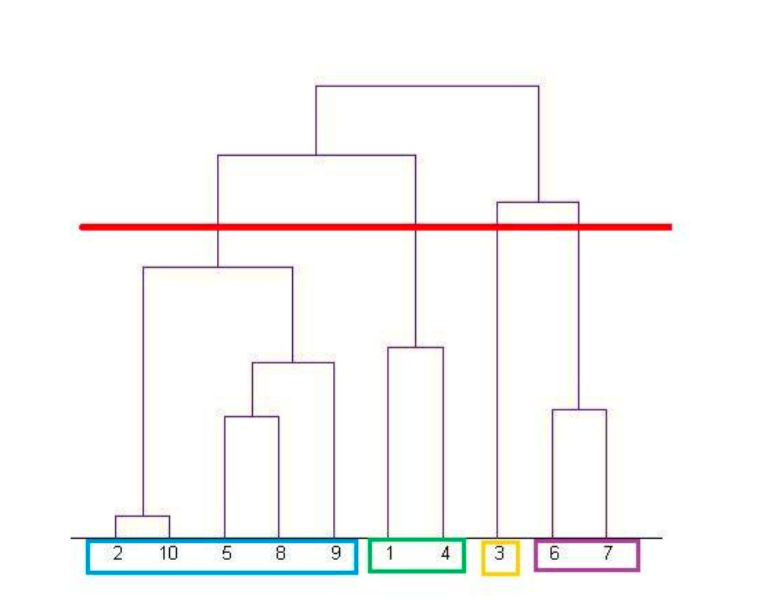
\includegraphics[scale=0.2]{dendrogram.png} \\
    Fig.1. Dendrogram cut example
\end{center}

\section{Community Detection Algorithms}

\subsection{Edge Betweenness Algorithm (Girvan-Newman) (2002)}

Girvan and Newman proposed the first algorithm in 2002 that made community detection feasible. Before then, the technique that was used to detect communities was to try to maximize the value of the quality function that was described by simple definitions which was oftenly an NP- complete problem. \\

Girvan and Newman proposed a value for each edge called edge-betweenness value so that the edges that connect communities will have higher edge-betweenness scores and edges that are inside the communities will have lower edge-betweenness scores\cite{raghavan}. \\

They defined edge-betweenness as the total number of shortest paths that are passing over that edge. According to this definition, the inter-cluster edges have more shortest paths passing through them and therefore yielding higher edge-betweenness scores. Then the algorithm simply removes the edges with high edge-betweenness scores to isolate communities from each other\cite{raghavan}. The algorithm is as follows: \\

\begin{enumerate}
\item Calculate betweenness scores of edges as follows:
\begin{enumerate}
\item Assign all betweenness scores of edges to 0.
\item Do a Breadth First Search starting from a vertex V to find number of shortest paths to each of the other vertices.
\item Assign to each edge a local betweenness score depending on the number of shortest paths that pass through that edge. Add that score to the betweenness score of that edge.
\item Repeat this process for each vertex, accumulating the betweenness score of the edges.
\end{enumerate}
\item Remove the edge with highest edge-betweenness score.
\item Repeat this process until no edges left.
\end{enumerate}

Calculating the betweenness score is done from scratch after each removal, so it is costly. However, since it goes on until there are no edges left, it can generate a full dendrogram at the end of its execution. Let’s say we have the following graph at the start. Calculating edge betweenness for vertex E:

\vspace{15ex}

\begin{figure}
    \centering
    \subfloat[Fig.2. Initial Graph]{{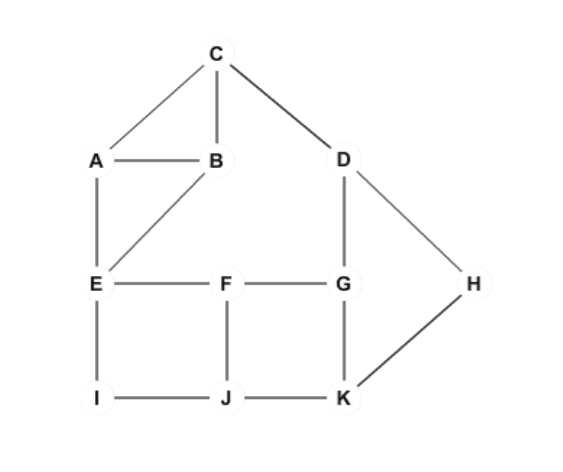
\includegraphics[width=5cm]{gn1.png} }}%
    \qquad
    \subfloat[Fig.3. Graph after BFS starting from vertex E ]{{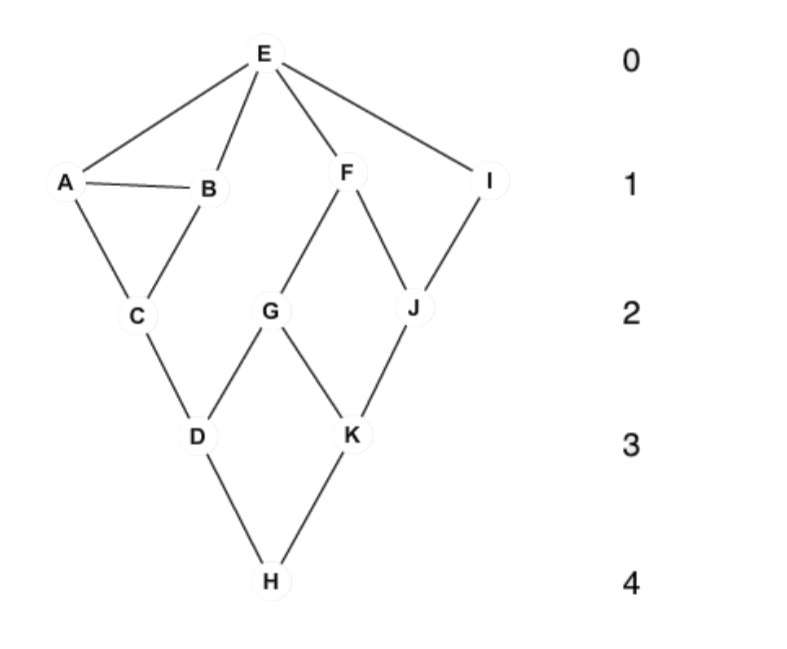
\includegraphics[width=5cm]{gn2.png} }}%
\end{figure}

\begin{sidewaysfigure}
    \begin{tikzpicture}
        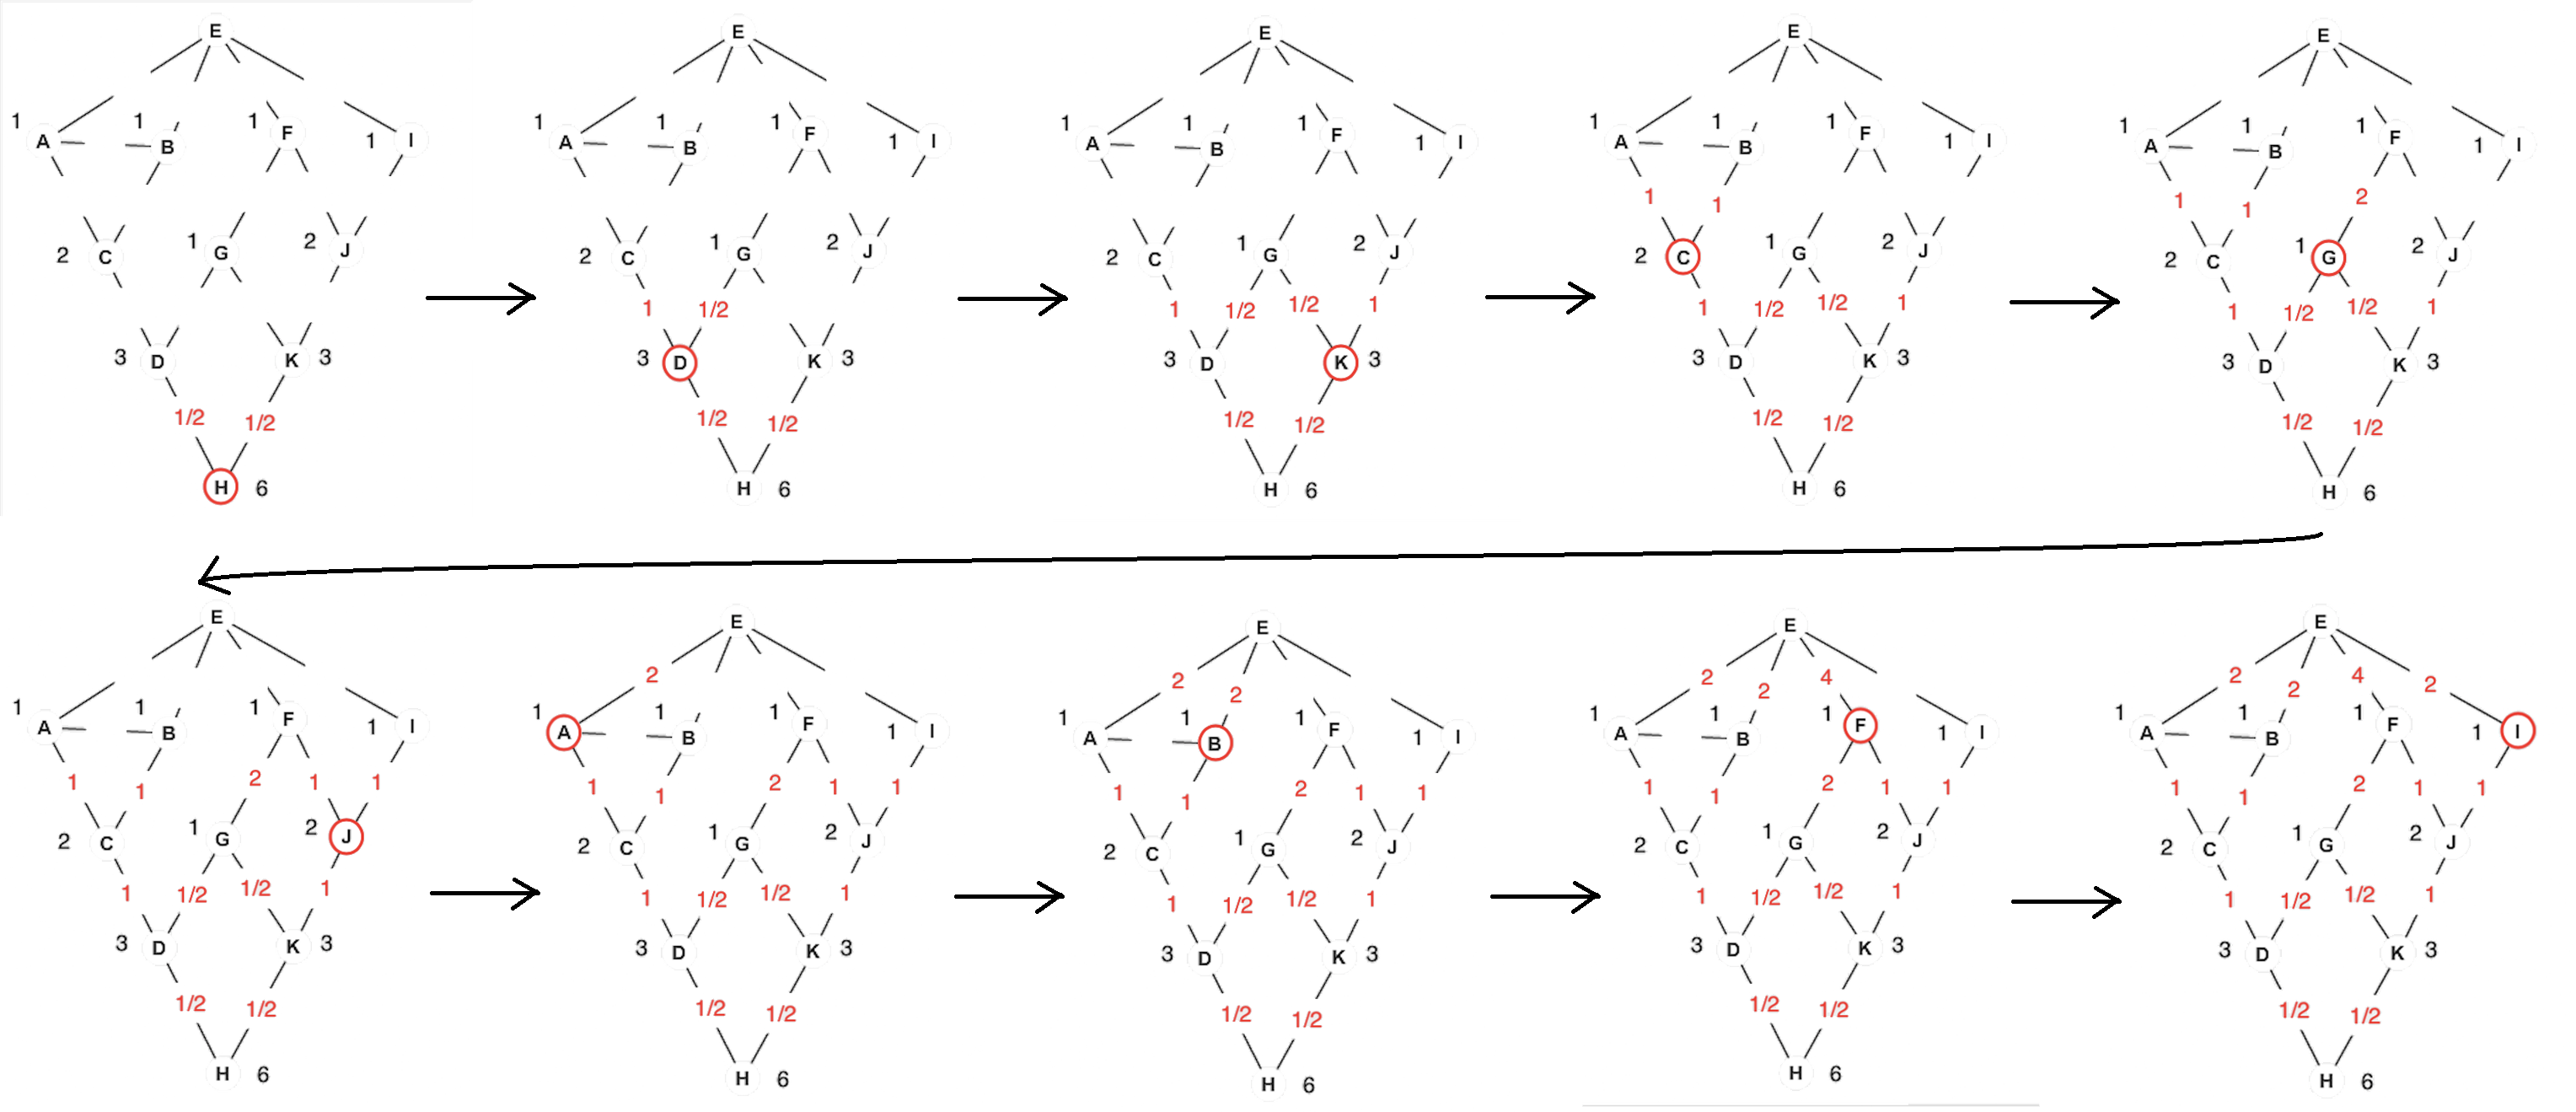
\includegraphics[scale=0.25]{gn3.png}  
    \end{tikzpicture}
    \caption{Fig.4. Computing Edge-Betweenness Contribution for vertex E}
    \label{fig:awesome_image}
\end{sidewaysfigure}


Due to the costly calculations of edge-betweenness after each removal of an edge with cubic complexity in total $O\left(|V||E|^2 \right)$, this algorithm is feasible for at most around a thousand vertices and a few thousand edges in today’s computational power. Also, this algorithm does not provide the information on where to cut the dendrogram; or in other words, the optimal point to stop removing the edges. One needs to define a quality function and check its value at each level of the dendrogram so that the maximum value of the quality function can be found. \\

\subsection{Walktrap Algorithm (Pons et al.) (2005)}

In this algorithm, we put a random walker on one of the vertices and let her roam for few steps. By definition of a community, as there are more edges inside the community with respect to between the communities, a random walker tends to get trapped inside its community in a graph. Using this fact, one can have an idea on the structure of a graph after multiple random-walks. \\

At start, all vertices are in separate communities (there are m communities in the graph where m is the number of vertices). Then, similar to the Topic-Specific PageRank calculations \cite{mmds}, a random walker starts at a random vertex V and walks around a number of steps. Running the random walks for each vertex, one gets a distance measure between each vertex pairs (i.e. edges that are in the graph)\cite{random}. Then the vertices with smallest distance between them are combined and merged communities are formed. Therefore, this algorithm runs in a bottom-up manner in contrast to Edge-Betweenness Algorithm which was previously discussed and was running in a top-down manner. \\

The length of a random walk is important since it determines the probability of each vertex being in that community of the starting vertex. Generally 3, 4 or 5 is picked for this value. The value chosen for the length of the random walk is dependent on the expected size of an average community in the graph. If the length of a random walk is relatively smaller than the size of a community, the random walker may never reach to some components of some communities, in which case undesired results may be reached. \\

The probability of going from vertex i to j in a given graph in t steps is distance between two vertices can be defined as follows: \\

\[ r_{ij} = \sqrt{ \mathlarger { \sum_{k=1}^{n} \frac{ \left( p_{ik}^{t} - p_{jk}^{t} \right)^{2} }{d\left( k \right) } } } \] \\

where the d(k) is the degree of vertex k. \\

Therefore, the
  This means to find the distance between vertex i and j, we first find the difference probability of (going from i to k) – (going from j to k) for all vertices k in the graph. Before we take the Euclidean Norm of those values, we divide each probability by the degree of the vertex k since the random walks might be entered to vertex k via any one of its edges.
After having a distance metric for two vertices, we define the probability of going from community C to a vertex j as follows: \\

\[ P_{Cj}^{t} = \frac{1}{|C|}  \mathlarger{ \sum_{i \in C} P_{ij}^{t} }  \] \\

This formula means that the probability of going to vertex j from community C is the average probability of going to vertex j from each vertex i within this community. \\

Lastly, having vertex-vertex distance and community-vertex probability, we define a community-community distance as follows: \\

\[ \mathlarger{ r_{C_{i}C_{j}} } = \sqrt{ \mathlarger { \sum_{k=1}^{n} \frac{ \left( p_{C_{i}k}^{t} - p_{C_{j}k}^{t} \right)^{2} }{d\left( k \right) } } } \] \\

This is the same distance formula defined above; but starting within communities instead of individual vertices. With the same line of thinking, the Euclidean Norm of the probabilities (from community i to vertex k) and (from community j to vertex k) are taken with the normalizer degree of vertex k; for all k. \\

Algorithm assigns each vertex to their individual communities at the start. Then computes values for vertices. At each time, the community j with the smallest distance to community i are
merged together to form a larger community. As this process continues, all communities are merged into one community and the dendrogram can be formed by taking each merge operation into account. \\

\subsection{Label Propagation Algorithm (Raghavan et al.) (2007)}

Label Propagation Algorithm is a relatively fast algorithm with respect to the previous algortihms discussed in this paper, but an unstable one. In this algorithm, each vertex is assigned a unique label at the start of the execution. Then, at each round, the vertices adopt the most-frequent label among their neighbors. As the rounds pass, the community structures in a graph will be filled with the vertices with same labels\cite{raghavan}. This algorithm does not depend on any a priori information about the graphs or the communities such as the number of expected communities, the central nodes of the communities and so on. The formal steps of the algorithm are as follows: \\

\begin{enumerate}
\item Initialize the labels for all nodes in the graph. For each vertex i, label at time 0 is $ L_i\left(i\right) = i$.
\item Start the first round. Set t = 1. 
\item Put all vertices in a random order R.
\item For each vertex $v \in R$ (in order), check the neighbors $N_{v}$of v and put the label f that is the most frequent onto v’s label. i.e. $ L_v\left(t\right) = f$ . In case of a tie, pick any one of them randomly.
\item If all nodes have the label of the most frequent label of their neighbors, end the algorithm. Otherwise, the next round starts. $t = t+1$.
\end{enumerate}

In graphs with strong community structures, this algorithm yields results fast\cite{raghavan}, but it is generally unstable and may result in different communities despite the same initial conditions. Due
to the randomized nature of ordering of the nodes and its randomized tie-breaking rule, the runtime and the resulting community structures are not trustable. Therefore, this algorithm is applied multiple times and the collected results are aggregated to get more stable results. \\

Another downside of this algorithm is that it does not necessarily converge into a set of communities in a finite amount of time. The following example is taken from Raghavan et al.’s paper where they demonstrate one of the divergent labeling situations. The algorithm may not stop at formations such as this one and the worst-case complexity of this algorithm is consequently $O(\infty )$. \\

\begin{center}
    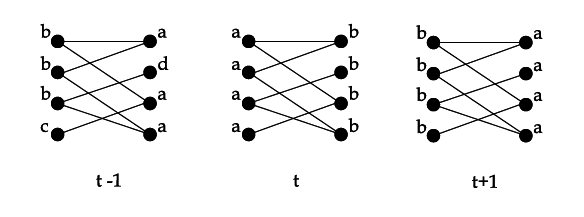
\includegraphics[scale=0.7]{labelPropLoop.png} \\
    Fig.4. After moment t, the labels on the left and right will be swapped at each iteration. The method is inconclusive. \cite{raghavan}
\end{center}

To test how good the community detection algorithms are, there is a famous graph called Zachary’s Karate Club graph in which there are overlapping communities and high number of nodes whose community classifications are hard and ambiguous. \\

Here are the different results of Label Propagation Algorithm on Zachary’s Karate Club graph from the original paper of Raghavan et al.: \\

\begin{center}
    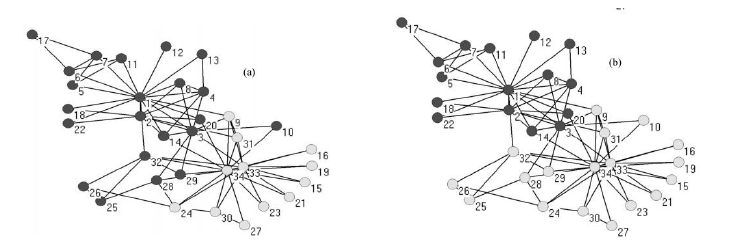
\includegraphics[scale=0.5]{labelPropKarateClub.png} \\
    Fig.5. Label Propagation Method on Zachary’s Karate Club yielding different results. The vertices with the same color are in the same community\cite{raghavan}.
\end{center}


When the algorithm terminates, two or more disconnected groups of nodes may have the same label. This happens when two or more neighbors of a node receive its label and pass the labels in different directions, which ultimately leads to different communities adopting the same label. In such cases, after the algorithm terminates, one can run a breadth-first search on the sub-networks of each individual group to separate the disconnected communities. This requires an overall time of O($m+n$) where m is the number of vertices and n is the number of edges. When aggregating solutions, disconnected groups within communities are rarely found. \\

\subsection{Louvain Method (Blondel et al.) (2008)}

Louvain Method is an algorithm that heuristically tries to maximize the modularity function Q. The algorithm, compared to the other algorithms in the field, runs very few number of operations for a given vertex to calculate the modularity change on all possible ways to include the given vertex to a community such that at least one of its adjacent vertices is in the community. \\

\[ Q\left(G\right) = \frac{1}{2m}  \sum_{all\ i,j} \left( A_{ij} - \frac{k_i k_j}{2m} \right)  \delta \left( C_i, C_j\right) \] \\

where is the degree of vertex k and m is the total number of edges in the graph. Here in this formula, \\

$A_{ij}$ is the element in the adjacency matrix representation of the graph. It has the value 0 if there is no connection between the vertices i and j; or weight of the edge as the value if the edge exists between i and j. This also means that the formula works regardless of graph’s being weighted or unweighted graph. \\

$ \mathlarger{ \frac{k_i k_j}{2m} } $ is the expected number of edges (or expected weight) between vertices i and j. This can be thought as follows: The vertex i has and vertex j has possible connections with the outside. Therefore, there exists possible $k_i * k_j$ connections in the null model for this edge to exist, among total of m edges. Also, keep in mind that if there exists an edge connecting vertex i and j, that edge occupies one degree from both of their degrees and thus we count it twice. Therefore, we also need to divide it by 2 to get the expected number of edges between those two nodes. \\

As a result, $\left( A_{ij} - \frac{k_i k_j}{2m} \right)$ measures how strongly i and j are connected with respect to the null model of this graph. \\

$\delta \left( C_i, C_j\right)$ is the delta function, also called Kronecker’s Delta which is simply 1 when two vertices are
in the same community and 0 otherwise. It tells us that when the term next to it, i.e. $\left( A_{ij} - \frac{k_i k_j}{2m} \right)$ is positive, we should take vertex j and put it into the community of vertex i so that the total modularity shall increase; whereas if that term is negative, the two vertices should stay separated. \\

$\frac{1}{2m}$ is a normalizing constant which makes Q between the values -1 and 1.
In the way that it tries to maximize the modularity function of the graph, Louvain Method is very similar to another greedy algorithm, proposed by Clauset et al. in 2004, but differs in the way while Clauset et al.\cite{clauset}. method retains the modularity variations of each vertex pair in a max-heap, Louvain Method merges nodes belonging to the same community into a one “supervertex” at the cost of accuracy and stability\cite{blondel}. \\

The algorithm can be expressed in three steps, which are repeated until convergence as follows: \\

\begin{enumerate}
\item Initialize each vertex to be a distinct community.
\item For each vertex A, consider each of the adjacent vertices to A and evaluate the modularity gain from removing A from its original community and including A in the community of the adjacent vertex. Find the vertex adjacent to A that \textbf{maximizes the modularity} gain and add A to its community.
\item Standing for all the vertices belonging to the same community, create a \textbf{supervertex} to replace the community while maintaining all the edges to the other supervertices. Maintain the number of edges from the all the vertices of community C to all the vertices of community D by weighing the edges between the supervertices of the new graph for the modularity gain calculation in the next iteration. 
\end{enumerate}


Louvain Method has a bottom-up approach, similar to the Walktrap Algorithm which discussed above, where each node is initially marked to be a unique community and communities are formed with the merging of other communities during the following iterations of the algorithm such that each merge operation can be traced back to reveal a dendrogram structure of the communities to detect the different communities at desired levels. \\

\begin{center}
    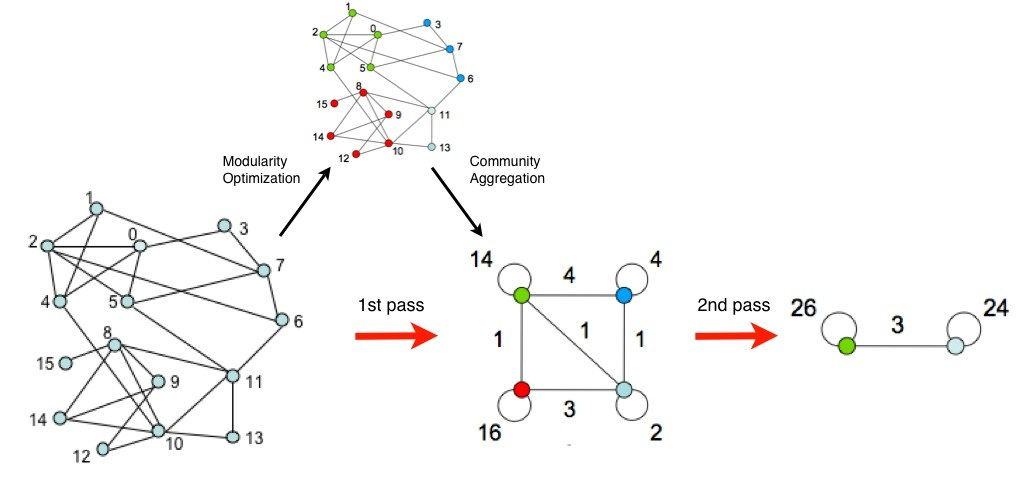
\includegraphics[scale=0.35]{louvain.jpg} \\
    Fig.6. Consecutive Iterations of Louvain Method\cite{blondel} \\
\end{center}

One important remark about the algorithm is the order the vertices are selected to be merged with a community directly affects the result, there could be some vertices between strong community components, such vertices may be decided to be added to different communities on the basis of how many vertices have already been merged in the respective communities. In such cases the algorithm may yield different results on different runs. \\

Nonetheless, the algorithm’s hastiness to evaluate the fate of a vertex enables it to detect the communities in very large graphs that other algorithms fail to evaluate in tolerable lengths of time. The algorithm’s complexity is dependent on the number of vertices that are evaluated with their adjacent vertices for modularity gain, however, the number of vertices the algorithm has to evaluate depends on the structure of the graph itself effective from the second iteration where the supervertices, whose number is not known, are evaluated. \\

This algorithm is one of the first algorithms that worked under reasonable runtime with massive data-sets. Rather than computation time like previous algorithms, this algorithm limited by the size of the main memory for the storage of the network and this algorithm made it possible to work with more than 100 million nodes. Actually, Louvain method outperforms many similar modularity optimization methods in terms of both modularity and runtime, according to the paper of Aynaud et al.\cite{french}. \\

\section{Recent Developments and Open Research Problems}

\subsection{Finding Overlapping Communities and Finding Maximum K-Clique Problem}

As it was stated previously, a vertex does not necessarily belong to only one community in a graph. Actually, in most of the cases, we will have nodes that are inside multiple communities. In such cases, we would also like to identify such edges in our graph that are overlapping between communities. \\

The former algorithms mostly proposed methods that were yielding one community for one node. However, with the start of social networking era, overlapping communities especially drew people’s attention. In 2005, Palla et al. proposed an algorithm for finding overlapping communities with the name of \textbf{ K-Clique Percolation Method } or sometimes \textbf{ Clique Percolation Method (CPM) }. To understand how this method works, we must have an apriori information on cliques. \\

A K-clique is a \textbf{complete graph} with K vertices. All K vertices are connected to each other fully. E.g. a 3-clique is a triangle.
Two K-Cliques are \textbf{adjacent cliques} if they have (K - 1) mutual vertices. \\

Lastly, \textbf{K-Clique community} is the union of all adjacent cliques that can be reached from each other in a chain-like manner. \\

\begin{figure}[h]%
    \centering
    \subfloat[Fig.7. Adjacent Cliques with K = 3]{{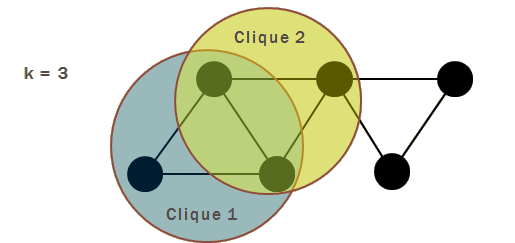
\includegraphics[width=5cm]{adjacentCliques.png} }}%
    \qquad
    \subfloat[Fig.8. Adjacent Cliques combined.]{{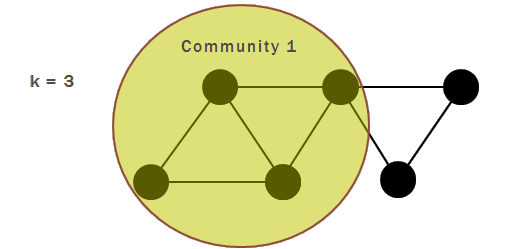
\includegraphics[width=5cm]{cliqueCommunity.png} }}%
\end{figure}

In Clique Percolation Method, the algorithm tries to find K-cliques in the graph first. Then, for each K-clique found, it considers all the edges except the chosen 1 of them to check if the former clique has an adjacent clique. If it has, the newly found K-clique and the previous set of adjacent cliques are unified to get the bigger community instance. This is repeated until there are no vertices belonging to a clique\cite{eleven}.
The motivation behind the algorithm is that the community structures tend to have K-cliques in them whereas it is unlikely to have a K-clique between two communities. By exploiting this fact, the algorithm adds all vertices that happen to be in one of the cliques in the community structure. In the resulting community structures, some of the vertices will be in multiple communities, creating the overlapping area between those communities. For the Zachary’s Karate Club, the algorithm yields this result: \\

\begin{center}%
    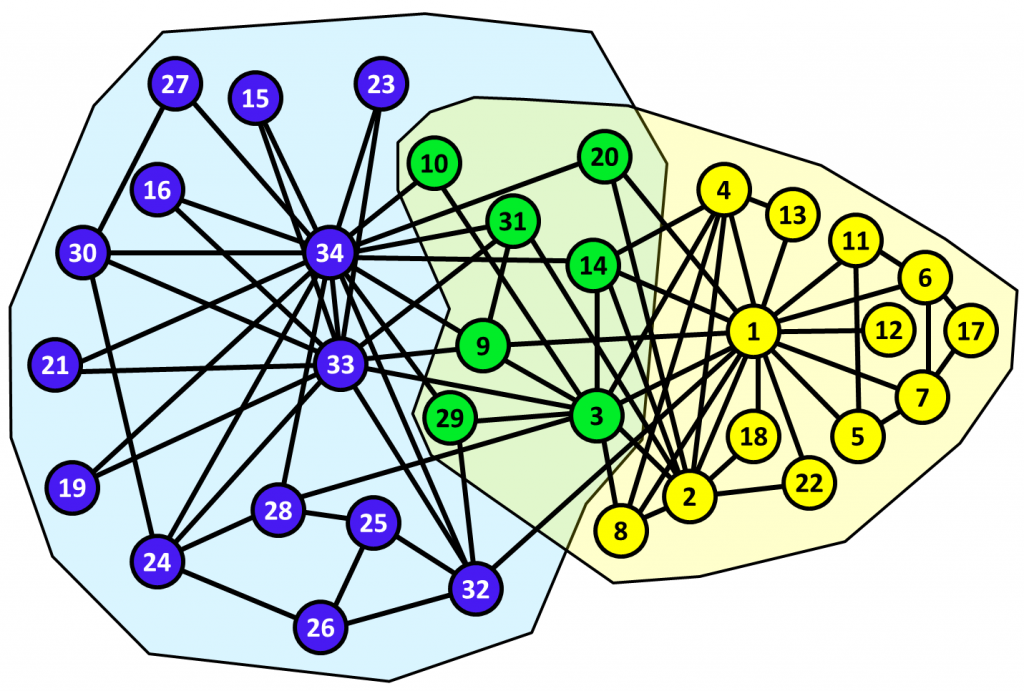
\includegraphics[scale=0.2]{karateclique.png} \\
    Fig.9. Zachary’s Karate Club partitioning with CPM 
\end{center}

One must keep in mind that the number K here cannot be too high. Mostly K=3 to 5 are used. Finding the first K-cliques in the graph is done by brute-force and as the number of vertices in the community increases, the time required to find all K-cliques in the graph becomes exponentially harder. In fact, the algorithm’s complexity is $O \left( 2^{n}\right)$ where n is the number of vertices \cite{eleven}. In fact, finding the maximum K-clique in a given graph is an NP-Complete problem \cite{clique}. \\

Finding the overlapping communities is still an ongoing research and many papers are being published each year to evaluate the problem and to find novel techniques to tackle the problem. For instance, Community-Affiliation Graph Model is developed by Yang-Leskovec in 2012 to model the overlapping communities and find a way to classify the vertices in overlapping communities \cite{overlapping}. \\

\subsection{Benchmarks}
One important open problem still have not been addressed by a consensus is how to evaluate the results of the community detection algorithms. A benchmark that has been accepted by all to compare various algorithms is not reality\cite{fortunato}. Most of the algorithms are only tested on a limited number and variety benchmarks which leave some vital details hidden and make it harder to comparatively investigate all the algorithms at once. In addition to already-in-use benchmark, which has 128 vertices divided into 4 groups of equal sizes, proposed by Girvan and Newman \cite{raghavan}, in 2009, LFR benchmark was proposed, which aimed to apply the Power Law distribution of networks in real life to its graphs so that the proposed algorithms could be tested to their limits and more could be known\cite{cdbible}. However, the issue remains unsolved, partly due to the fact that there is not a perfect quality function to measure how well a community detection algorithm should work and defining a benchmark, although the benchmarks are now better at representing real life network structures have simultaneously become more ambiguous to define in themselves well-partitioned communities \cite{fortunato}. \\

\section{Conclusion}

Community detection in graphs is a hot-topic. As the number of network structures increase in our daily lives, the importance of finding community structures in networks also continues to increase. As a result, new methods and new ideas are being developed on the subject matter everyday. As it has been discussed in this paper, some of the existing methods are reliable but slow whereas some of them are fast but unstable. Since the concept of communities is inherently vague and unclearly defined by its nature, there is no final answer/partitioning for the algorithms to reach. However, there exists some metrics such as modularity to evaluate the partitioning of the existing algorithms. \\

In recent years, new algorithms having promising results with almost linear running times (such as Louvain Method) have been developed and detecting communities have become more and more scalable. However, there are still issues related to grounding and evaluating a given partition and having a benchmark that is widely accepted/believed to be distinguishing. There is still no consensus on the qualitative definition of null models and overlapping communities \cite{fortunato}. Although we have algorithms with linear complexities, they mostly work in a greedy manner so that the resulting graphs are approximations of the desired solution in the end. Despite all these, one must grant that the exhaustive research efforts on the subject matter has improved the complexity of clustering algorithms by at least one order of graph size, in roughly a decade. As the subject matter grows more and more mature; and more number of researches conducted on the topic, it is only logical to assume that there will be linear-time algorithms that will yield the expected partitions for a given network structure in the future. \\

\begin{thebibliography}{40}

\bibitem{euler} Euler, L. (1741). Solutio problematis ad geometriam situs pertinentis. Commentarii academiae scientiarum Petropolitanae, 8, 128-140.

\bibitem{fortunato} Fortunato, S. (2010) "Community detection in graphs." Physics Reports 486.3. 75-174.

\bibitem{erdos} Erdős, P., \& Rényi, A. (1961). On the strength of connectedness of a random graph. Acta Mathematica Hungarica, 12(1-2), 261-267.

\bibitem{clauset} Clauset, A., Newman, M. E., \& Moore, C. (2004). Finding community structure in very large networks. Physical review E, 70(6), 066111.

\bibitem{mmds} Leskovec, J., Rajaraman, A., \& Ullman, J. D. (2014). Mining of massive datasets. Cambridge University Press.

\bibitem{random} Pons, P., \& Latapy, M. (2006). Computing communities in large networks using random walks. J. Graph Algorithms Appl., 10(2), 191-218.

\bibitem{blondel} Blondel, V. D., Guillaume, J. L., Lambiotte, R., \& Lefebvre, E. (2008). Fast unfolding of communities in large networks. Journal of Statistical Mechanics: Theory and Experiment, 2008(10), P10008.

\bibitem{raghavan} Raghavan, U. N., Albert, R., \& Kumara, S. (2007). Near linear time algorithm to detect community structures in large-scale networks. Physical Review E, 76(3), 036106.

\bibitem{gnr} Girvan, M., \& Newman, M. E. (2002). Community structure in social and biological networks. Proceedings of the national academy of sciences, 99(12), 7821-7826.

\bibitem{eleven} Palla, G., Derényi, I., Farkas, I., \& Vicsek, T. (2005). Uncovering the overlapping community structure of complex networks in nature and society. Nature, 435(7043), 814-818.

\bibitem{french} Aynaud, T., Blondel, V., Guillaume, J. L., \& Lambiotte, R. (2010). Optimisation locale multi- niveaux de la modularité.

\bibitem{clique} Bomze, I. M., Budinich, M., Pardalos, P. M., \& Pelillo, M. (1999). The maximum clique problem. In Handbook of combinatorial optimization (pp. 1-74). Springer US.

\bibitem{overlapping} Yang, J., \& Leskovec, J. (2012, December). Community-affiliation graph model for overlapping network community detection. In Data Mining (ICDM), 2012 IEEE 12th International Conference on (pp. 1170-1175). IEEE.

\bibitem{cdbible} Lancichinetti, A., \& Fortunato, S. (2009). Community detection algorithms: a comparative analysis. Physical review E, 80(5), 056117.

\end{thebibliography}



\end{document}
